\documentclass{main}
    

\usepackage{graphicx}      % include this line if your document contains figures
\usepackage{natbib}        % required for bibliography
\usepackage{enumerate}
\usepackage[utf8]{inputenc}
\usepackage{graphicx}
\usepackage{float}
\usepackage[centerlast,small,sc]{caption} 
\setlength{\captionmargin}{30pt}
\usepackage[brazilian]{babel}
\usepackage[none]{hyphenat} 
\usepackage{subcaption} 
\usepackage{capt-of}
\usepackage{kpfonts} 
\usepackage{stackengine}
\usepackage{calc}
\usepackage[hyphens]{url}
\usepackage{hyperref}
\hypersetup{breaklinks=true}
\usepackage{pdfpages}



\newlength\shlength
\newcommand\xshlongvec[2][0]{\setlength\shlength{#1pt}%
  \stackengine{-5.6pt}{$#2$}{\smash{$\kern\shlength%
    \stackengine{7.55pt}{$\mathchar"017E$}%
      {\rule{\widthof{$#2$}}{.57pt}\kern.4pt}{O}{r}{F}{F}{L}\kern-\shlength$}}%
      {O}{c}{F}{T}{S}}
\sloppy  

\begin{document}

\begin{frontmatter}

\title{Metodologia e revestimento robótico de turbinas \textit{in situ} - EMMA
\thanksref{footnoteinfo}} 

\thanks[footnoteinfo]{Contrato ESBR e COPPETEC JIRAU 09/15 6631-0003/2015 (ANEEL
R\&D program).}

\author[1]{Gabriel Alcantara C. S.}
\author[1]{Renan S. Freitas}
\author[1]{Eduardo Elael M. S.}
\author[1]{Estevão Fróes}
\author[2]{Julia Campana}
\author[1]{Ramon R. Costa}


  \address[1]{Departamento de Engenharia Elétrica, COPPE UFRJ, Rio de Janeiro,
  Brasil} 
  \address[2]{Departamento de Artes e Design, PUC, Rio de Janeiro}
  
\begin{abstract}                % Abstract of not more than 250 words.
%TODO Gabriel: Resumo
\end{abstract} 
 
\begin{keyword}
%TODO Gabriel: Keywords
\end{keyword}

\end{frontmatter}

\section{Introdução}
%TODO  Gabriel: contextualização do problema, sota, Jirau
\section{Metodologia}
%TODO Gabriel: metodologia da solução, etapas de desenvolvimento (pesquisa de
% mercado, sota, simulações, montagem e etc)


A metodoligia empregada durante o desenvolvimento do projeto EMMA consistiu em
diversas etapas, que alimentavam a seguinte e, caso necessário,
realimentavam uma etapa anterior para refinamento da solução ou alinhamento de
resultados. Primeiramente, no EMMA-SOTA foi realizado uma pesquisa e delimitação
do escopo do problema, etapa fundamental para o completo entendimento do problema e
responsável por direcionar o esboço das primeiras soluções. 

Neste documento será verificada a viabilidade da utilização do manipulador MH12,
confirmando que é possível a total cobertura da pá durante o processo de
revestimento. A análise cinemática, dinâmica serão realizadas com o auxílio de
ferramentas de simulação como a plataforma OpenRAVE. Em seguida a estratégia de
controle e planejamento de trajetória assegura que a movimentação do manipulador
se desevolva de forma contínua em todo o espaço de juntas e que as velocidades e
acelerações máximas sejam respeitadas.

A análise detalhada de cobertura da pá, fornece os requisitos mínimos que a base
mecânica deve obedecer, como forças exercedidas e graus de liberdade necessários
para alcancar todas as posições da base do manipulador. A partir dos conceitos
analisados no EMMA-DETAIL, pode-se comparar diferentes soluções e as vantagens
de desvantagens de cada uma. Foi escolhido o conceito
Prismático-Rotacional-Prismático-Prismático (P-R-P-P) porque mostrou-se a
solução mais viável construtivamente. Foi realizado então o projeto básico da
solução e o dimensionamento dos componentes. Os resultados do dimensionamento
permitirão o detalhamento final da base mecânica, compra de materiais, montagem
e testes.





Solução mecanica

Conceito PRPP trilho primario transporte e trilho secundario posicionamento de
coating

Construcao - material, apoio, ancoragem, montagem e desmontagem

Dimensionamento - elementos finitos, tensoes forcas e momentos

Calibracao - reconhecimento do robo com marcadores
reconhecimento da pa correspondence grouping
simulacao de dados 


\section{Solução do sistema de controle}
%TODO Renan: solução do sistema de controle com simulações
\section{Solução mecânica}
%TODO Estevão: solução final, detalhada  da mecanica com possiveis simulações

A solução de revestimento de uma pá de turbina \textit{in situ} requer um robô
de pequeno a médio porte, capaz de passar pelo limitado acesso da turbina. 
No entanto, a pá da turbina é uma peça com uma grande área a ser coberta e
nenhum manipulador comercial que atenda ao requisitos citados é capaz de
alcançar, de uma só posição, toda a sua extensão.
Assim, é necessário prover ao robô liberdade de posicionamento para realizar o
revestimento em pequenas regiões da pá, por posição de base.

Devido ao peso do manipulador e por questões de segurança, a sua movimentação no
interior da turbina não pode ser uma tarefa manual. Logo, uma base mecânica deve
ser capaz de levar o robô desde a escotilha até a posição ideal para o
revestimento, de forma segura e precisa. O dimensionamento desta base deve levar
em consideração todos os esforços de operação, como: o peso do sistema; as
cargas dinâmicas de movimentação do robô e o empuxo da pistola.

Foram estudados diversos conceitos para os graus de liberdade providos pela
base mecânica. O estudo destes conceitos estão detalhados no EMMA-DETAIL.

\subsection{Conceito}

A escolha do conceito da solução foi baseada nos graus de liberdade da base
mecânica para permitir ao robô movimentação e alcance necessários para realizar 
o revestimento. 

O conceito aqui aprofundado é denominado P-R-P-P, ou
Prismático-Rotacional-Prismático-Prismático.
A seguir estão descritas cada junta que compõe a base.

\begin{itemize} 

	\item\textbf{Prismática 1:} A primeira junta prismática é formada por um
	trilho, sobre uma estrutura modular. Este trilho é denominado ''trilho
	primário'' e está paralelo ao eixo da turbina, indo desde a escotilha de
	entrada até a região posterior da pá, próxima ao distribuidor.

	\item\textbf{Rotacional:} A segunda junta, rotacional, é formada por um
	eixo apoiado sobre mancais de rolamento e une o trilhos ''primário'' à segunda
	junta prismática, denominada trilho ''secundário''.

	\item\textbf{Prismática 2:} A terceira junta,
	prismática, é formada por um trilho (secundário), também
	sobre uma estrutura modular. Este trilho é posicionado paralelo ao plano
	transversal da pá, e permitirá ao robô os deslocamentos laterais ao longo de
	toda a extensão da largura da pá. 

	\item\textbf{Prismática 3:} A última junta, prismática, é formada por um
	macaco mecânico tipo sanfona, com curso mínimo de $200~mm$, permitindo ao robô
	maior alcance em altura.
	
\end{itemize}

A figura~\ref{fig::conceito} apresenta o conceito descrito.

\begin{figure}[h!]
	\centering
	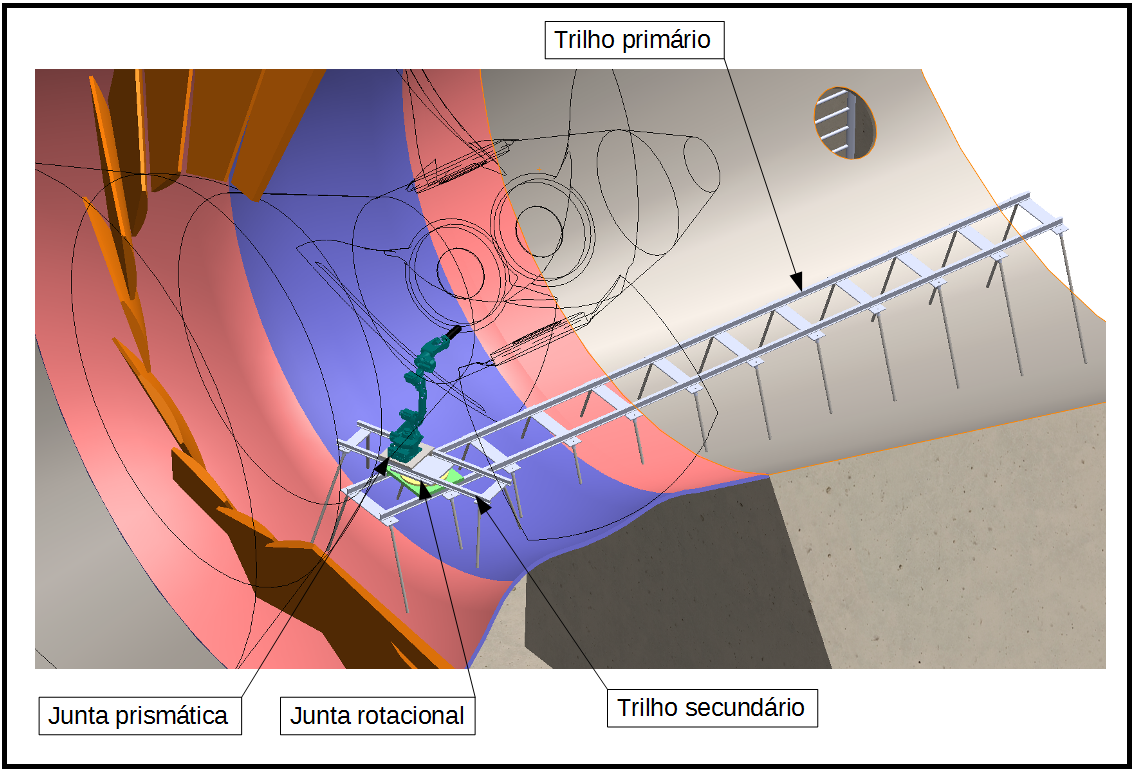
\includegraphics[width=0.9\columnwidth]{figs/conceito/conceito_P-R-P-P_01_tags}
	\caption{Conceito P-R-P-P da base mecânica}
    \label{fig::conceito}
\end{figure}

Neste conceito, o manipulador é movimentado pelo trilho primário até a região
próxima a pá. Em seguida é montado o trilho secundário a partir da base onde o
manipulador está fixado. A orientação do trilho secundário é definida pela
movimentação da junta rotacional entre os trilhos primário e secundário. A
partir daí, o manipulador pode ser movimentado ao longo do trilho secundário e
posicionado para o revestimento. Para as regiões de difícil alcance será
utilizada a junta de elevação.

\subsection{Construção}

\subsubsection{Trilho e carrinho}

Para movimentação e posicionamento precisos do manipulador foi selecionado o
sistema de trilho perfilado e carrinho de rolamento de esferas recirculantes. 
O trilho selecionado tem o perfil segundo a norma ISO 12090-1 e o carrinho segue
a norma DIN 645-1. 
Estes componentes são próprios para aplicações nas quais se requer grande
capacidade de carga e precisão de posicionamento.

\begin{figure}[h!]
	\centering
	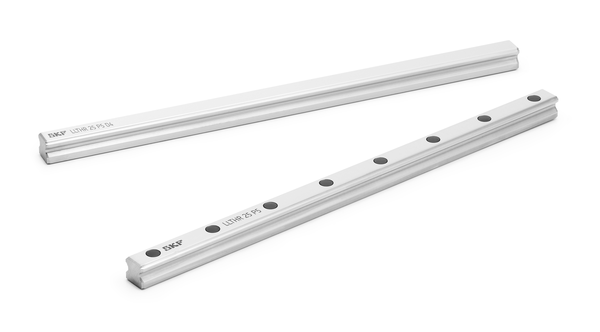
\includegraphics[width=0.7\columnwidth]{figs/construcao/trilho_LLT}
	\caption{Trilho para movimento linear}
    \label{fig::trilho}
\end{figure}

\begin{figure}[h!]
	\centering
	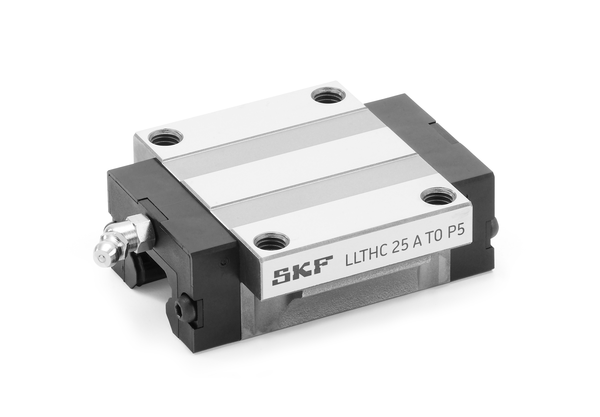
\includegraphics[width=0.7\columnwidth]{figs/construcao/carrinho}
	\caption{Carrinho de esferas recirculantes}
    \label{fig::carrinho}
\end{figure}

Estes componentes permitem algumas opções de montagens que variam de acordo com
a aplicação. 
Estas opções vão desde a utilização de um único trilho e único carrinho,
montagens com 1 trilho e 2 carrinhos, e até 2 trilhos e 4
carrinhos, como mostrado na figura~\ref{fig::sist_2por4}.

\begin{figure}[h!]
	\centering
	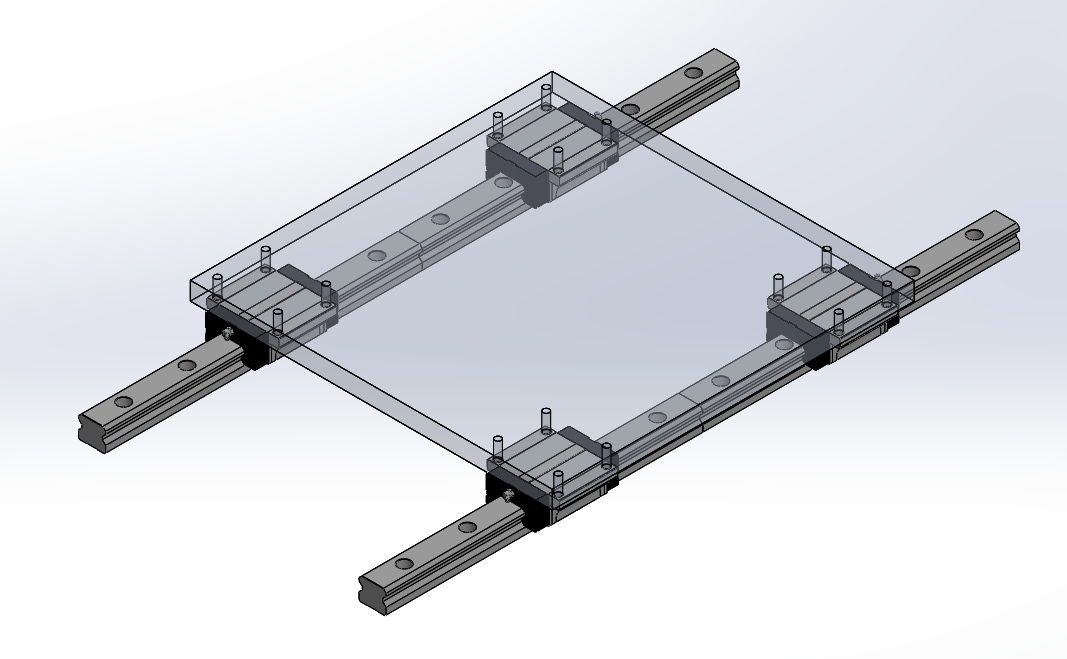
\includegraphics[width=0.9\columnwidth]{figs/construcao/sist_2por4}
	\caption{Montagem com 2 trilhos e 4 carrinhos}
    \label{fig::sist_2por4}
\end{figure}

As cargas promovidas pelo manipulador são elevadas, sobretudo na base, que
reage às cargas distantes do ponto de fixação, causando momentos elevados. 
A vantagem da utilização de mais de um carrinho por trilho é a possibilidade de
anular-se os momentos de reação nos carrinhos, na direção ortogonal ao eixo do
trilho. 
No caso da solução proposta, as cargas são variáveis em sua magnitude e direção.
Por esta razão, a configuração que utiliza 2 trilhos e 4 carrinhos é a mais
indicada, já que os carrinhos ficam livres de reagirem a momentos e as cargas ficam
dividas em mais componentes.

%---------------------------------------------------------------------
\subsubsection{Perfil de alumínio estrutural} \label{sec::perfil}

A estrutura que servirá de base para o trilho deve ter como prinicipal
característica a modularidade. Devido à geometria variável do ambiente no
interior da turbina, é necessário também que esta estrutura permita 
flexibilidade de montagem dos apoios e ancoragens ao longo do trilho.
Cada módulo da estrutura será composto pelo perfil de alumínio estrutural, a
partir de onde serão fixados o trilho e os acessórios de apoio e ancoragem da
estrutura no ambiente.
Tais módulos devem permitir transporte e montagem manuais, de forma fácil e
rápida.
Por isso, optou-se pelo perfil de alumínio estrutural. Este perfil possui
ranhuras para fixação de componentes padronizados e permite a construção
de uma grande variedade de estruturas funcionais de geometrias simples ou
complexas.

\begin{figure}[h!]
	\centering
	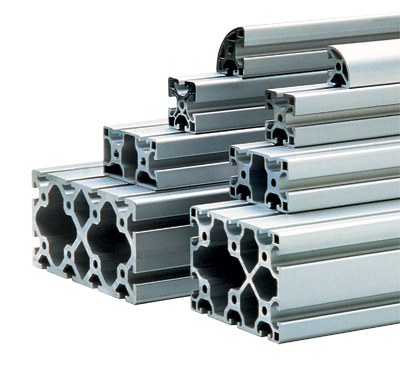
\includegraphics[width=0.7\columnwidth]{figs/construcao/aluminio_estrutural}
	\caption{Perfis de alumínio estrutural}
    \label{fig::aluminio_estrutural}
\end{figure}

A figura~\ref{fig::modulo_primario_explod} apresenta um exemplo de um dos módulos do
trilho primário, a partir da montagem deste no perfil de alumínio
estrutural. Este módulo pode ser repetido ao longo do eixo longitudinal do
trilho, formando assim a estrutura completa. 
Para se ajustar ao ambiente da turbina, há variação apenas do comprimento dos
pés de apoio e dos braços de ancoragem, mantendo-se as mesmas dimensões de todos
os outros componentes.

\begin{figure}[h!]
	\centering
	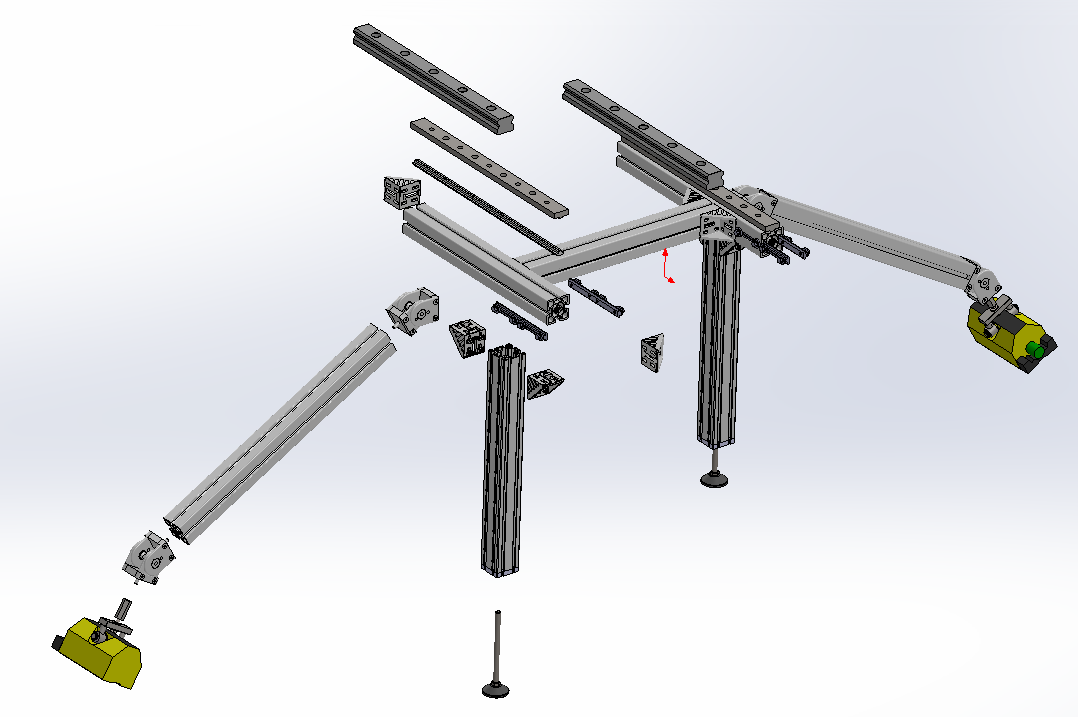
\includegraphics[width=0.9\columnwidth]{figs/construcao/Modulo_Explodida_01}
	\caption{Vista explodida de montagem com perfil de alumínio estrutural}
    \label{fig::modulo_primario_explod}
\end{figure}

%---------------------------------------------------------------------
\subsubsection{Pés de apoio}

Os pés de apoio da estrutura primária têm o objetivo de nivelar o trilho no
ambiente, permitindo que a estrutura possa formar um plano horizontal e paralelo
ao eixo da turbina. Devido às inclinações da superfície do túnel e do
aro-câmara, os pés de apoio devem permitir graus de liberdade que compensem
algum desvio. Além disto, o comprimento de cada ''perna'' da base varia ao
longo da estrutura, sendo necessário permitir uma margem de erro de
montagem a partir de uma regulagem de seu comprimento.

Foi verificado que o maior ângulo formado entre o eixo horizontal e a superfície
da turbina é de aproximadamente $9^{\circ}$. Optou-se portanto por pés com
interface do tipo rótula, exemplificado na figura~\ref{fig::spindle}, que
permitem até $10^{\circ}$ de inclinação entre a haste e à base, além de $75~mm$ de regulagem
do comprimento, por meio da rosca da haste. %TODO Conferir Estevao

\begin{figure}[h!]
	\centering
	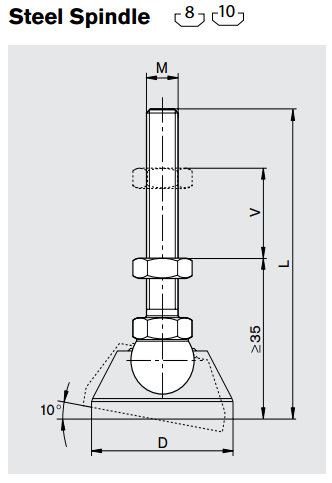
\includegraphics[width=0.4\columnwidth]{figs/construcao/spindle}
	\caption{Pé com junta rotular entre a haste e a base}
    \label{fig::spindle}
\end{figure}

%---------------------------------------------------------------------
\subsubsection{Ancoragem}

A ancoragem da estrutura é importante para prevenir movimento da base quando o
robô estiver em movimento. Sua principal função é tornar a base rígida o
suficiente para que as deformações elásticas e vibrações da estrutura não
interfiram na precisão requisitada para o processo de revestimento.

Os braços de ancoragem são constituídos de duas juntas rotacionais em cada
extremidade. Estas juntas permitem que o braço se ajuste à superfície da
turbina, posicionando as bases magnéticas na orientação ideal para o acoplamento
magnético. A figura~\ref{fig::ancoragem} apresenta os braços de ancoragem ao
longo da estrutura.

\begin{figure}[h!]
	\centering
	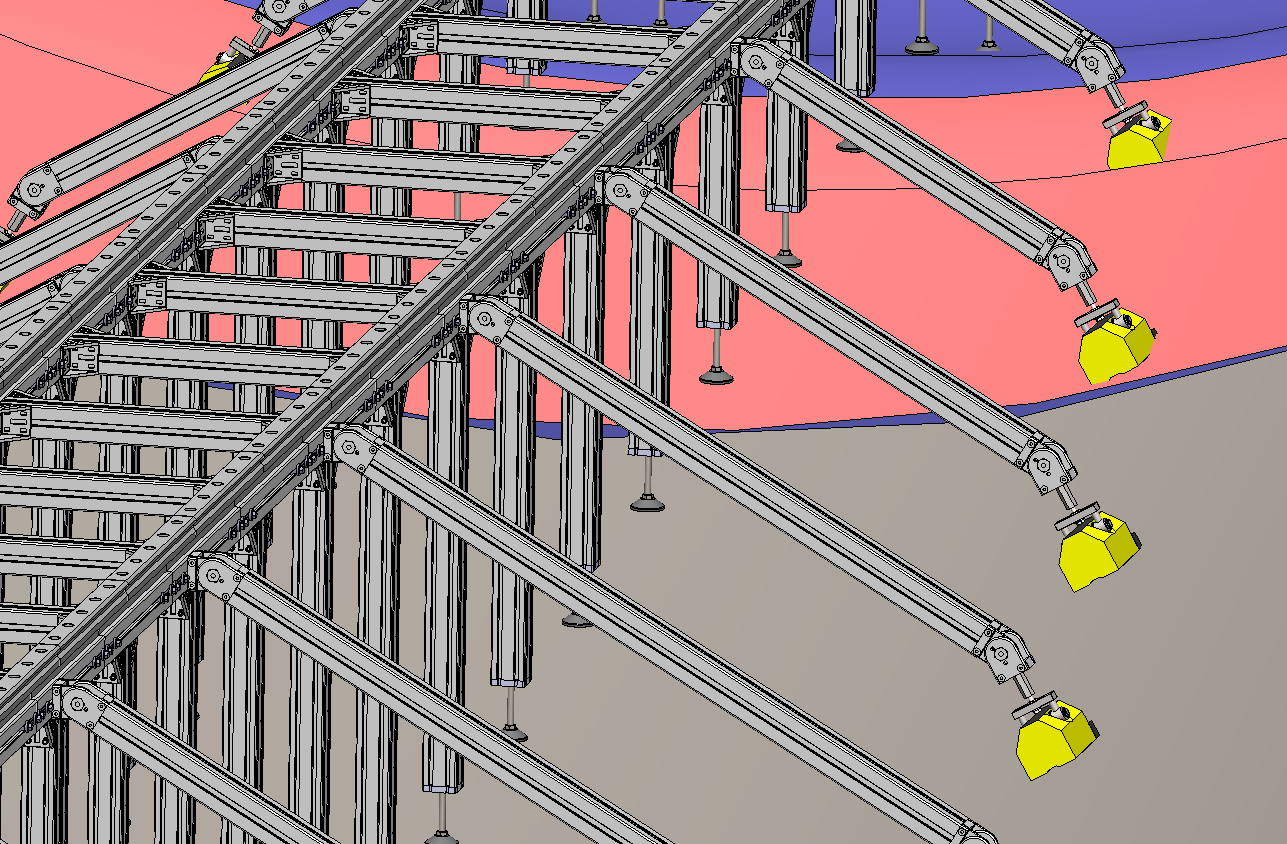
\includegraphics[width=0.9\columnwidth]{figs/construcao/ancoragem}
	\caption{Braços de ancoragem do trilho primário}
    \label{fig::ancoragem}
\end{figure}

%---------------------------------------------------------------------
\subsubsection{Bases magnéticas}

As bases magnéticas são equipamentos comerciais cuja principal aplicação na
indústria é o içamento e movimentação de peças metálicas. Este equipamento é
composto por imãs permanentes que são alinhados através de uma alavanca em sua
carcaça. Desta forma, é possível controlar as linhas de campo magnético,
tornando a base atrativa magneticamente somente quando se desejar.

As bases magnéticas são os elementos de fixação não-permanentes que serão
utilizados para ancoragem da estrutura no ambiente da turbina. Foram realizados
testes para verificação da carga máxima suportada e o resultado foi
satisfatório e apresentado na seção de Apêndice B do EMMA-DETAIL.



\begin{figure}[h!]
	\centering
	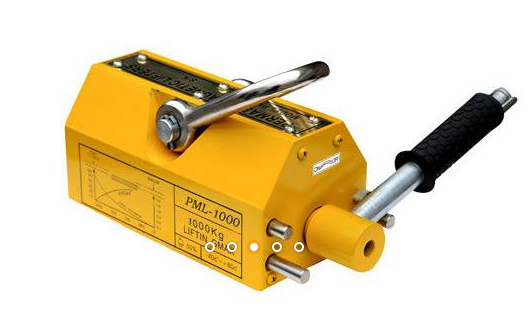
\includegraphics[width=0.5\columnwidth]{figs/construcao/base_magnetica}
	\caption{Base magnética para ancoragem}
    \label{fig::base_magnetica}
\end{figure}

%---------------------------------------------------------------------
\subsubsection{Junta de rotação}

A junta de rotação é composta por uma plataforma de posicionamento angular
horizontal.
O princípio de funcionamento é através de um par de engrenagens sem-fim e coroa,
em que e o acionamento do sem-fim pode ser feito por um volante com marcação de
ângulo. Este equipamento é muito utilizado em máquinas fresadoras verticais,
sendo denominado ''mesa divisora'' nesta aplicação.
Este equipamento atende às exigências de robustez, rigidez e precisão destas
máquinas operatrizes, portanto mostra-se ideal para a aplicação na base mecânica
da solução robótica de revestimento. A figura~\ref{fig::rotary_table} apresenta
uma mesa divisora com acinoamento manual e sistema sem-fim e coroa.

\begin{figure}[h!]
	\centering
	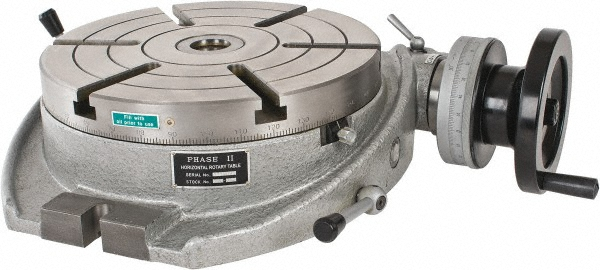
\includegraphics[width=0.6\columnwidth]{figs/construcao/rotary_table}
	\caption{Plataforma de rotação}
    \label{fig::rotary_table}
\end{figure}

%---------------------------------------------------------------------
\subsubsection{Junta de elevação}

Estudo apresentado no EMMA-DETAIL mostrou que para alcançar as regiões da pá
mais próximas ao rotor, e garantir a qualidade ideal de revestimento, é
necessária a elevação da base do manipulador em pelo menos $200~mm$.
Para realizar esta tarefa será utilizado um macaco mecânico do tipo sanfona.
Este equipamento foi escolhido devido ao seu tamanho compacto quando retraído,
$85~mm$, e um curso grande de elevação, $245~mm$. Seu acionamento é manual a
partir da rotação de uma alavanca conectada a uma barra roscada.
Para facilitar a manipulação desta junta, será adaptado um volante no
acionamento.
Um conjunto de cilindros e guias garantem o movimento preciso da junta e
robustez, transmitindo os esforços diretamente para a estrutura e prevenindo que
estes atuem no macaco mecânico.

\begin{figure}[h!]
	\centering
	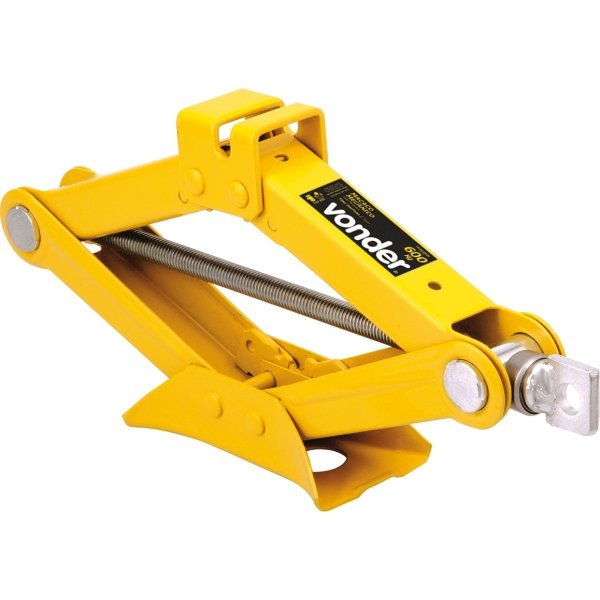
\includegraphics[width=0.6\columnwidth]{figs/construcao/macaco_sanfona}
	\caption{Macaco mecânico do tipo sanfona}
    \label{fig::macaco_sanfona}
\end{figure}

%---------------------------------------------------------------------
\subsubsection{Montagem}

A montagem da base mecânica no interior da turbina é feita a partir de módulos
(ou submontagens que formam elementos básicos de uma montagem maior). O exemplo
de um módulo da estrutura primária foi apresentado na
figura~\ref{fig::modulo_primario_explod}, na seção~\ref{sec::perfil}. 

A ideia neste conceito é que a estrutura possa ser montada a partir de um módulo
incial que se repete ao longo de uma mesma direção até formar-se a estrutura
completa. A montagem deve ser prática e rápida, assim como a desmontagem e
deve permitir a correção de pequenos erros de posicionamento no
ambiente a partir de ajustes simples. Por exemplo, se a posição do módulo
inicial estiver errada, pode-se ajustar o comprimento dos pés de apoio e a
posição dos braços de amarração facilmente. Isto é importante principalmente
devido a dificuldade de se estabelecer uma referência precisa no interior da
turbina e também devido a pequenas diferenças de projeto ou construção entre uma
turbina e outra.



Neste conceito, primeiro monta-se a estrutura e trilho
primário, e então, monta-se a base do manipulador no trilho primário. Esta base
contém os elementos que permitem os graus de liberdade de rotação e prismático
(elevação) e também serve de origem para a montagem da estrutura e trilho
secundário. 

\begin{figure}[h!]
	\centering
	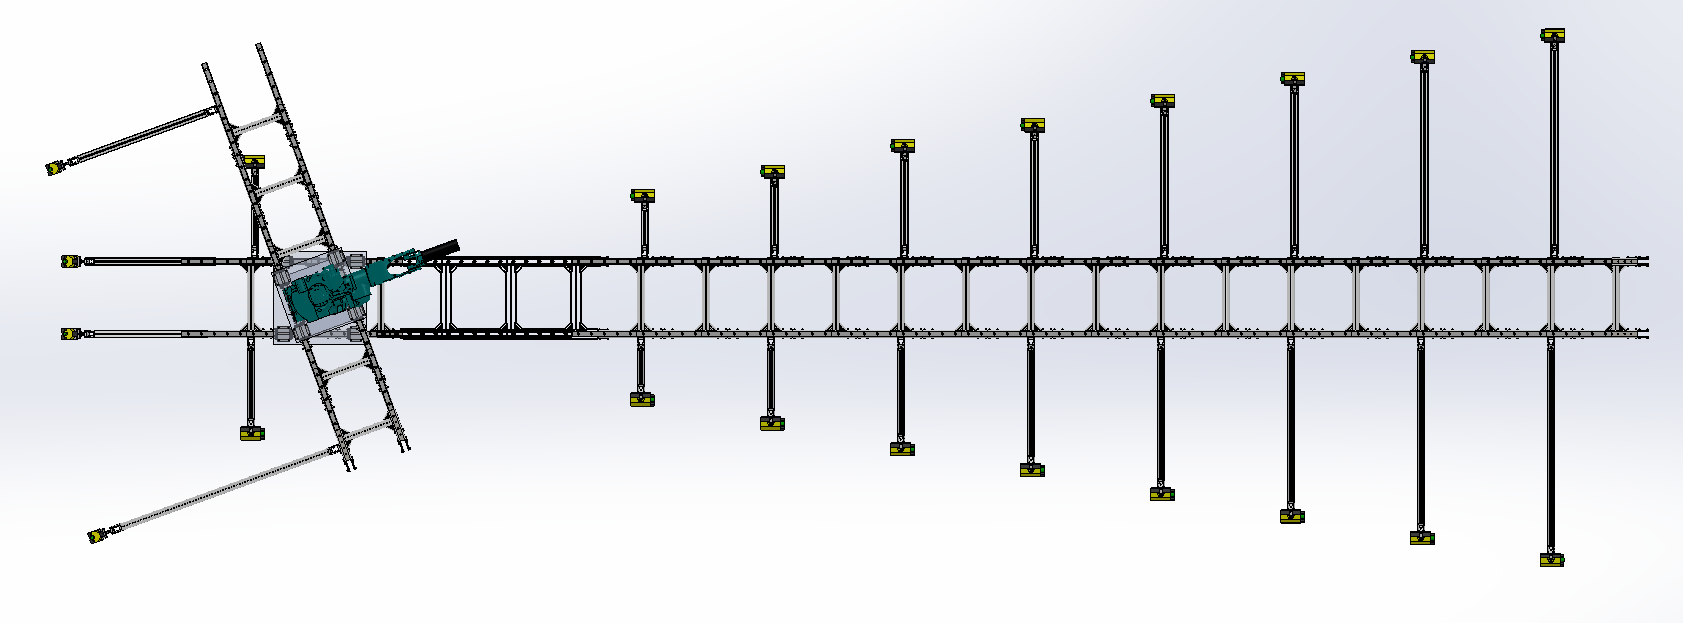
\includegraphics[width=0.9\columnwidth]{figs/construcao/EMMA_Base_Secundaria_04}
	\caption{Montagem da base mecânica}
    \label{fig::EMMA_Base_Secundaria_04}
\end{figure}

A figura~\ref{fig::EMMA_Base_Secundaria_04} apresenta uma vista superior da
montagem da base mecânica e a figura~\ref{fig::EMMA_Base_Secundaria_01}
apresenta a montagem no interior da turbina, em uma configuração de operação na
face posterior da pá. Nota-se que é necessária a desmontagem de parte do trilho
primário para posicionar a pá no melhor ângulo em relação à base. Esta é mais
uma vantagem de se ter um conceito modular para a estrutura.

\begin{figure}[h!]
	\centering
	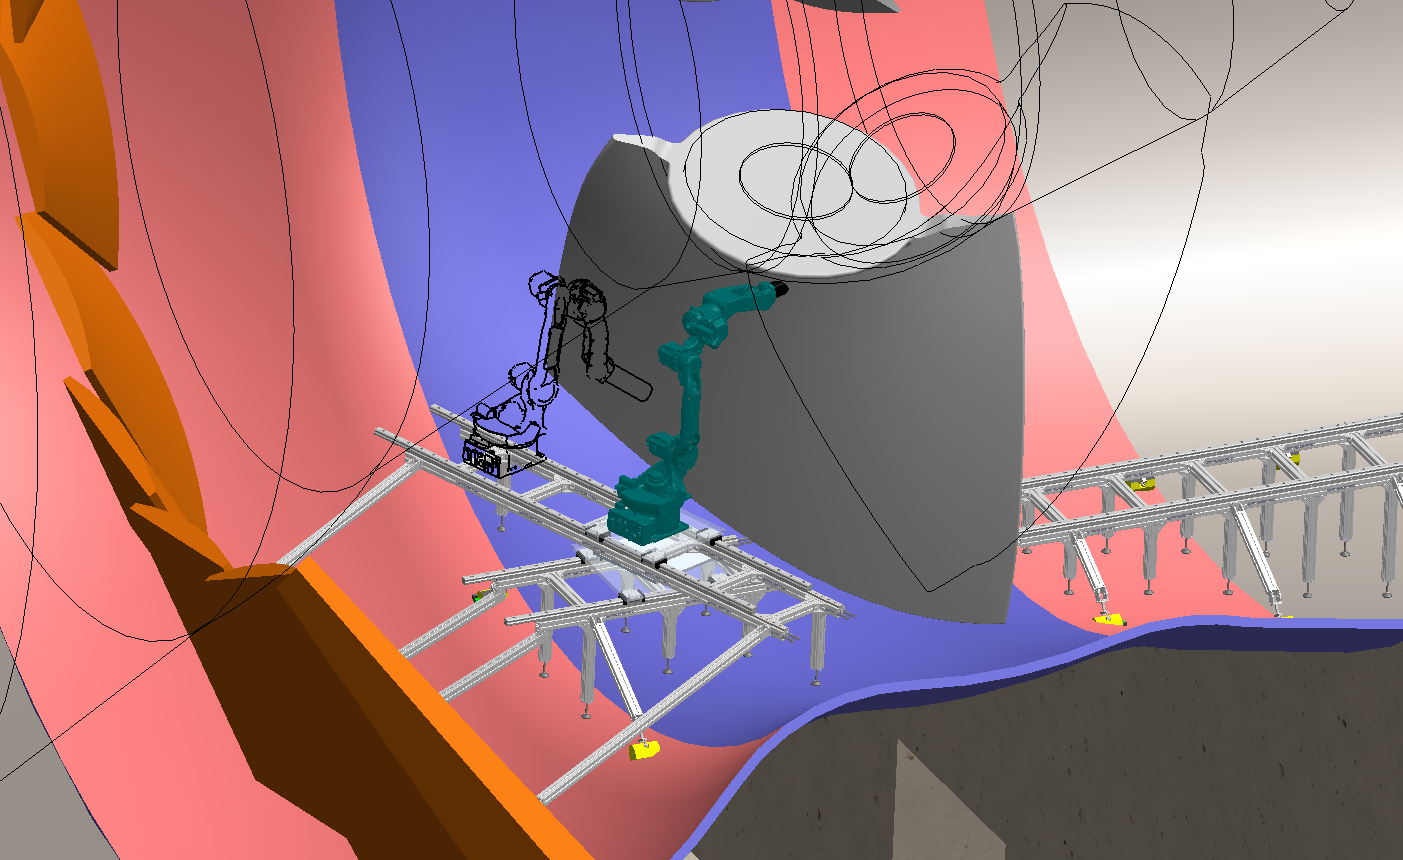
\includegraphics[width=0.9\columnwidth]{figs/construcao/EMMA_Base_Secundaria_01}
	\caption{Montagem da base mecânica no interior da turbina}
    \label{fig::EMMA_Base_Secundaria_01}
\end{figure}

%---------------------------------------------------------------------
\subsection{Dimensionamento}

O dimensionamento dos equipamento é a etapa que define diversos parâmetros, tal
que se destacam: a escolha de materiais; dimensões e geometria do projeto.
É a etapa compreendida entre o conceito ou projeto básico e o detalhamento que
permitirá a compra dos materiais e construção do protótipo. Nesta
etapa são verificados e calculados esforços estruturais, a integridade dos
equipamentos e avaliados, por exemplo tensão, Fator de Segurança (FS),
deslocamentos e deformações resultantes. A seguir são apresentados os cálculos
de dimensionamento dos equipamentos estruturais da base mecânica.

\subsubsection{Trilho}

Para o conjunto trilho-carrinho, foi utilizada a ferramenta de cálculo
\textit{SKF Linear Guide Calculator} da fabricante SKF (disponível em:
\url{http://www.skf.com/us/knowledge-centre/engineering-tools/skflinearguidescalculator.html}),
que permite o dimensionamento considerando os piores cenários de carregamento,
com forças e momentos máximos aplicados ao trilho.
O programa analisa toda a gama de dimensões dos trilhos do tipo LLT, fornecendo
o Fator de Segurança obtido para cada opção de tamanho.

O critério escolhido para seleção do trilho baseia-se no Fator de Segurança, que
deve ser maior ou igual a 2 ($FS\geq2$). 

Um relatório com o resultado de saída do programa encontra-se no Apêndice~\ref{append::skf}. 
Neste relatório estão apresentados os resultados de força resultante em cada
carrinho e o Fator de Segurança para algumas opções de montagem trilho-carrinho,
nos tamanhos 30 a 45. Dentre as opções, as que apresentaram resultado dentro do
critério de Fator de Segurança foram LLTHS 45 com sufixos U, A, R, LU, LA e LR.
Esta designação refere-se apenas ao carrinho que pode ter algumas variações de
tamanho e configuração de montagem. O conjunto trilho-carrinho selecionado foi
portanto o LLTHS 45 A, que apresenta FS igual a $2,1$ além de ser a opção padrão
do fabricante, tendo vantagens de disponibilidade e custo.
%TODO TODOS: Corrigir numeração do Apêndice na compilação

%---------------------------------------------------------------------
\subsubsection{Estrutura}

Com o objetivo de verificar as tensões devido às cargas do manipulador e também
verificar os deslocamentos por deformação elástica na base, foi feito um modelo
para análise da estrutura. Este modelo foi resolvido pelo Método de
Elementos Finitos utilizando o programa Autodesk\textregistered{}
Nastran\textregistered{} In-CAD.

A partir dos resultados, pode-se determinar alterações de geometria ou seleção
de materiais, que garantam maior segurança e rigidez da estrutura.
A seguir, são detalhados os parâmetros da simulação de Elementos Finitos.

\textit{Malha:} A análise foi modelada com elementos unidimensionais
de tamanho global de $25~mm$, e ordem quadrática.  E foram atribuidas propriedades
de viga, relativas ao perfil de alumínio estrutural, tais como:
momentos de inércia, momento de inércia polar e área de seção tranversal.

\textit{Material:} O material utilizado é o alumínio EN AW-6060
(norma~\cite{DIN_2007}) e foi definido no modelo a partir de suas propriedades físicas e mecânicas.

\begin{center}
\centering
\begin{tabular}{|l|l|l|}
\hline
\textbf{Propriedade}   & \textbf{Valor}   & \textbf{Unidade}  \\ \hline
Massa específica       & $2700$           & kg/m³             \\ \hline
Módulo de Elasticidade & $70,0$           & GPa               \\ \hline
Módulo de Cisalhamento & $26,1$           & GPa               \\ \hline
Coeficiente de Poisson & $0,34$           &                   \\ \hline
Limite de Escoamento   & $200$            & MPa               \\ \hline
\end{tabular}
\captionof{table}{Propriedades do EN AW-6060}
\label{tab::prop_material}
\end{center}


\textit{Condições de Contorno:} Na extremidade onde está acoplada a base
magnética dos braços de ancoragem, foram definidas restrições de translação
em todas as direções e rotação livre. Para os pés de apoio, definiu-se restrição
de translação apenas na direção do eixo $y$. A interface entre os trilhos
primário e secundário foi modelada utilizando elementos unidimensionais rígidos, fixados na
mesma posição dos carrinhos de rolamento.

A figura~\ref{fig::contorno} apresenta o modelo de análise da estrutura para o
robô posicionado na face posterior da pá. Estão representados o Sistema de
Coordenadas do modelo, a malha, as condições de contorno e os conectores
utilizados.

\begin{figure}[h!]
	\centering
	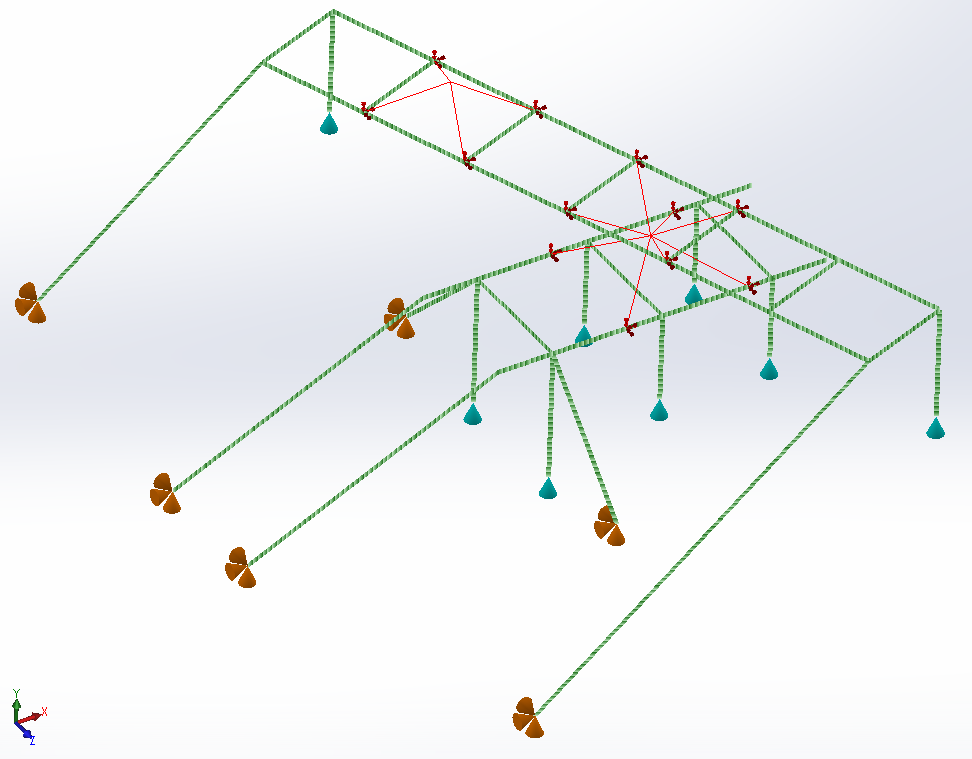
\includegraphics[width=0.9\columnwidth]{figs/dimensionamento/contorno}
	\caption{Malha e condições de contorno}
    \label{fig::contorno}
\end{figure}

\textit{Carregamento:} O carregamento utilizado para simulação
refere-se às forças e torques máximos atingidos pelo manipulador MOTOMAN modelo MH12, em
sua base. Este carregamento está de acordo com o manual de instalação e
manutenção do robô (\cite{MH12_manual}) como forças e torques de parada de
emergência.

\begin{center}
\centering
\begin{tabular}{|l|l|l|}
\hline
\textbf{Carga}		   & \textbf{Valor} & \textbf{Unidade}   \\ \hline
Força em X		       & 9025           & N	                 \\ \hline
Força em Y			   & -5885          & N                  \\ \hline
Força em Z			   & 9025           & N                  \\ \hline
Momento em X		   & 4120           & Nm                 \\ \hline
Momento em Y		   & 4120           & Nm                 \\ \hline
Momento em Z		   & 4120           & Nm                 \\ \hline
\end{tabular}
\captionof{table}{Forças e torques na base do robô}
\label{tab::carregamento}
\end{center}

As forças foram aplicadas através de um conjunto de conectores rígidos a partir
do ponto que representa o ponto de origem da base do robô. São $4$ conectores
representando a posição de cada carrinho no trilho secundário. Foram testadas
algumas posições do carrinho sobre o trilho para definir o pior caso.
Verificou-se que este ocorre quando o carrinho está a uma distância de
$817,5~mm$ a partir do eixo de rotação entre os trilhos. 
A figura~\ref{fig::carregamento} mostra a representação do carregamento na
direção resultante.

\begin{figure}[h!]
	\centering
	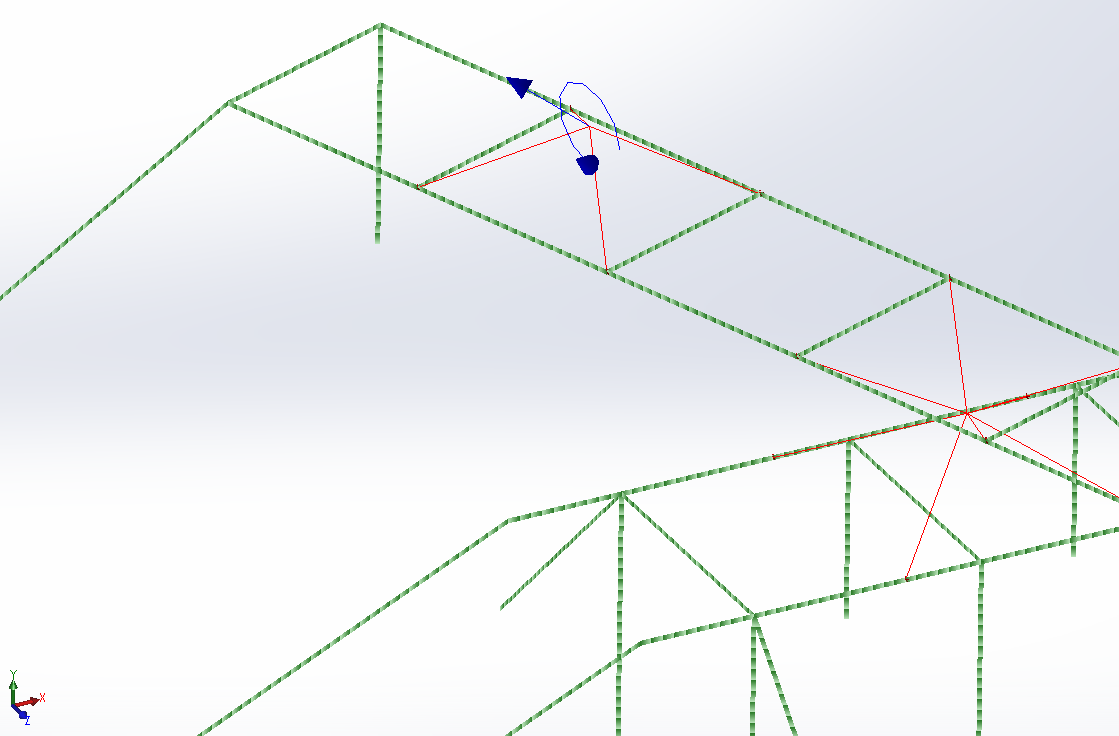
\includegraphics[width=0.9\columnwidth]{figs/dimensionamento/carregamento}
	\caption{Forças e torques na direção resultante}
    \label{fig::carregamento}
\end{figure}


\textit{Resultados:}

Abaixo são apresentados os resultados das simulações realizadas para a o modelo
da configuração de revestimento da face posterior da pá. 
A figura~\ref{fig::von_mises}, apresenta o resultado das tensões de Von Mises, 
emonstrando que o maior encontrado é $5,78~MPa$.

\begin{figure}[h!]
	\centering
	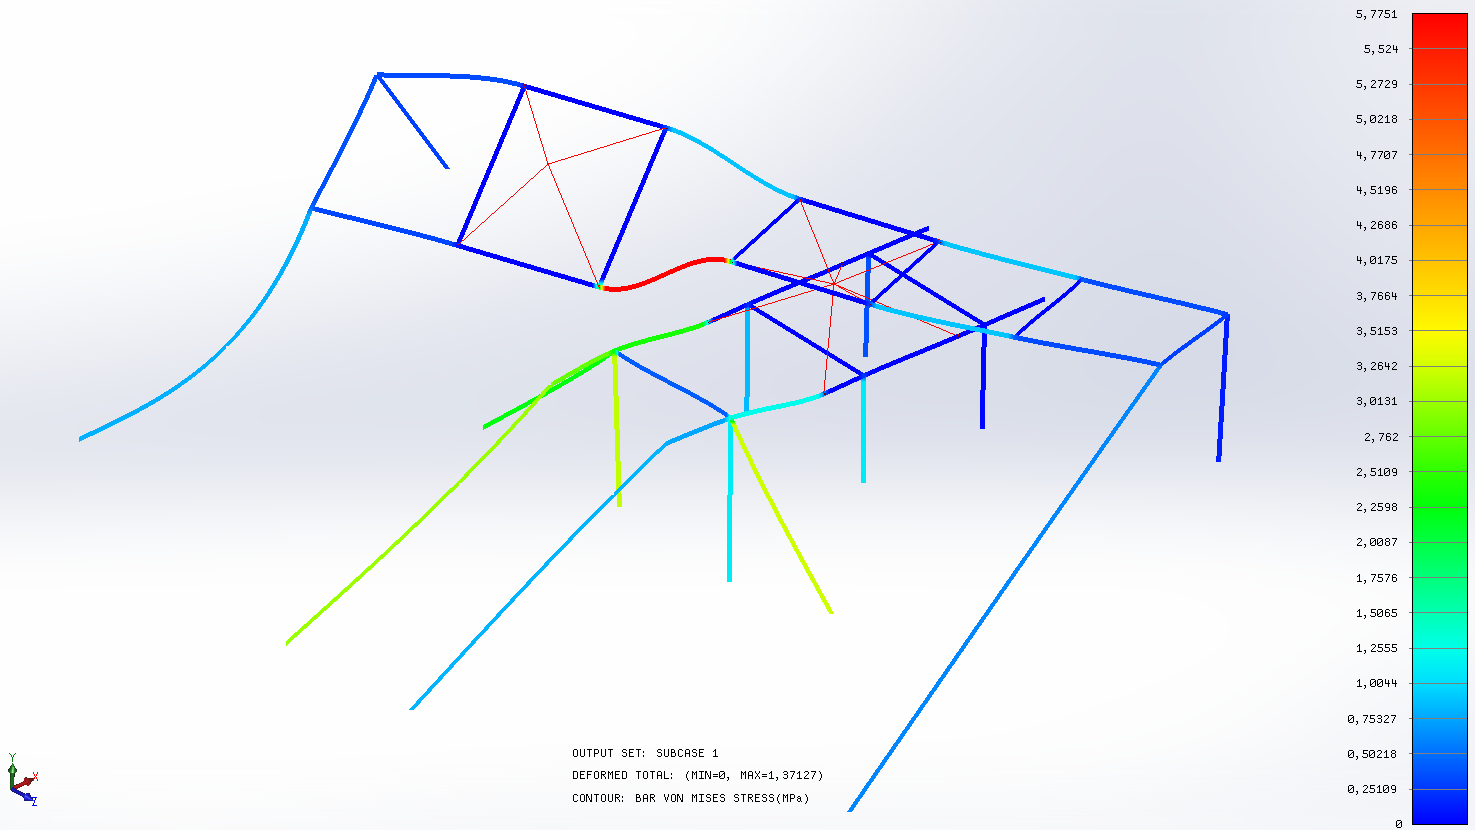
\includegraphics[width=0.9\columnwidth]{figs/dimensionamento/von_mises}
	\caption{Resultado de Tensões de Von Mises na estrutura, escala exagerada de
	deformação}
    \label{fig::von_mises}
\end{figure}

O Fator de Segurança pode ser calculado a partir da equação: 

\begin{equation*}
	FS=\frac{\sigma _y}{\sigma _{max}}
\end{equation*}

onde $\sigma_y$ é o Limite de Escoamento do material e $\sigma_{max}$ é a tensão
máxima encontrada. Assim, o Fator de Segurança é $34,6$.

O deslocamento máximo na estrutura está demonstrado na
figura~\ref{fig::deslocamento} e verifica-se que o valor do deslocamento
resultante na base do manipulador foi de $0,47~mm$.

\begin{figure}[h!]
	\centering
	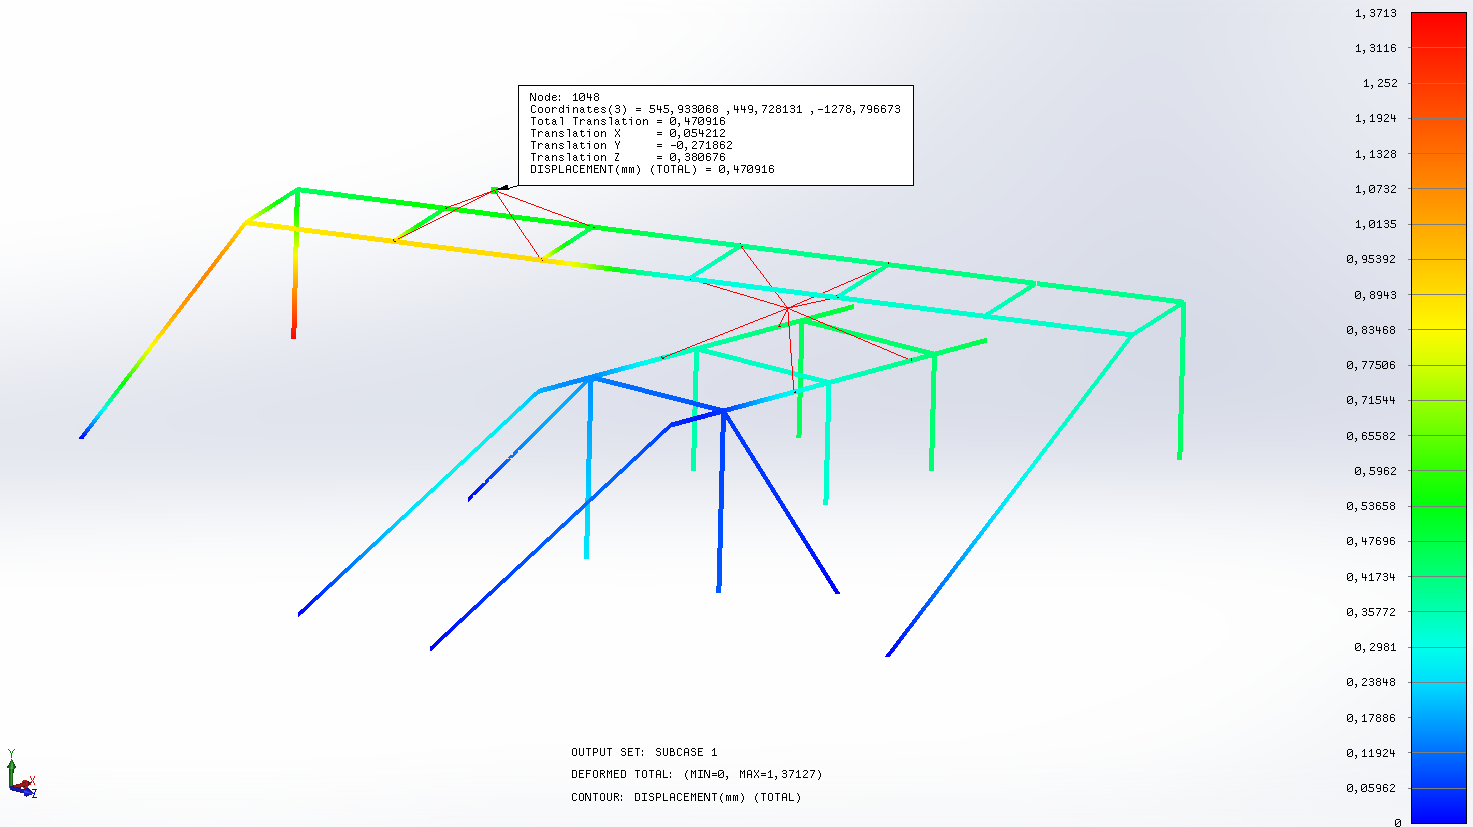
\includegraphics[width=0.9\columnwidth]{figs/dimensionamento/deslocamento}
	\caption{Resultado de Deslocamento Resultante na estrutura, escala real de
	deformação}
    \label{fig::deslocamento}
\end{figure}


As forças de reação nos braços de ancoragem são importantes para o
dimensionamento da base magnética. A tabela~\ref{tab::reacao_ancoragem}
apresenta os resultados encontrados em cada braço. A
figura~\ref{fig::mapa_forcas} apresenta a referência de cada braço de
ancoragem, de acordo com a tabela~\ref{tab::reacao_ancoragem}.

\begin{figure}[h!]
	\centering
	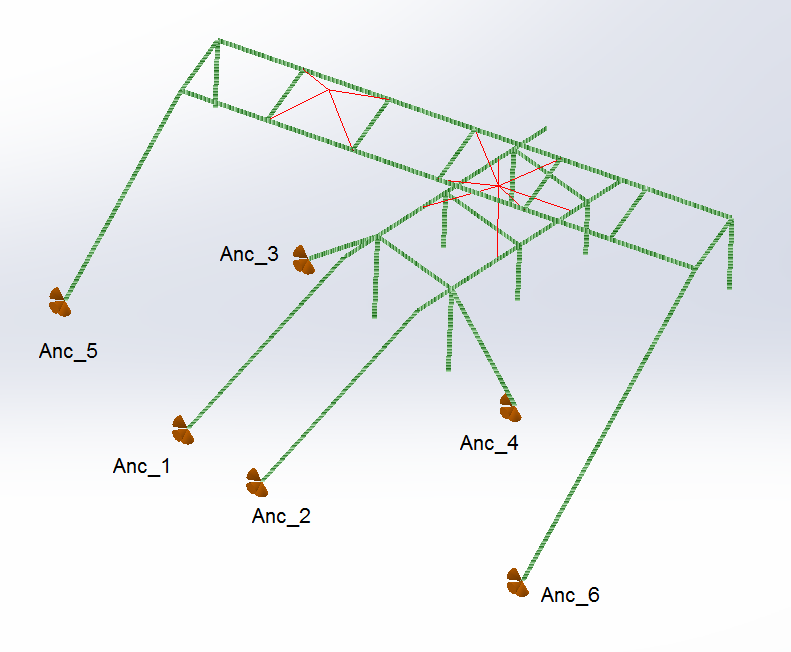
\includegraphics[width=0.8\columnwidth]{figs/dimensionamento/mapa_forcas}
	\caption{Referência dos braços de ancoragem para os resultados da
	tabela~\ref{tab::reacao_ancoragem}}
    \label{fig::mapa_forcas}
\end{figure}

\begin{center}
\centering
\begin{tabular}{|c|c|c|c|}
\hline
\textbf{Braço}  & \textbf{Fx {[}N{]}} & \textbf{Fy {[}N{]}} & \textbf{Fz {[}N{]}} \\ \hline
\textbf{Anc\_1} & -1678               & -1966               & 39                  \\ \hline
\textbf{Anc\_2} & -3433               & -4076               & 40                  \\ \hline
\textbf{Anc\_3} & 131                 & 206                 & -569                \\ \hline
\textbf{Anc\_4} & -9556               & 6621                & 6037                \\ \hline
\textbf{Anc\_5} & -1566               & -1436               & 1461                \\ \hline
\textbf{Anc\_6} & 651                 & 160                 & -254                \\ \hline
\end{tabular}
\captionof{table}{Forças de reação em cada ponto de ancoragem}
\label{tab::reacao_ancoragem}
\end{center}

Os resultados \textit{Fx}, \textit{Fy} e \textit{Fz} referem-se às forças
resultantes nas direções \textit{x,y,z} do sistema de coordenadas local de cada
braço de ancoragem. Neste sistema de coordenadas, a direção \textit{x} está
alinhada com o eixo longitudinal de cada braço de ancoragem e as direções
\textit{y,z} são as direções ortogonais a \textit{x}. 
Desta forma, os resultados negativos em \textit{x} indicam tração do
braço de ancoragem e os positivos, compressão.

%---------------------------------------------------------------------
\subsubsection{Base Magnética}

O dimensionamento das bases magnéticas está diretamente relacionado ao resultado
das forças resultantes em cada braço de ancoragem, já que são estes os elementos
que representam as restrições no modelo de Elementos Finitos.

Assim, deve-se comparar o resultado da tabela~\ref{tab::reacao_ancoragem} com a
capacidade máxima de carga da base magnética comercial. Para aceitar a base
magnética escolhida, deve-se respeitar as seguintes relações:

 \begin{equation*}
	|F_{x}|\leq\frac{2}{3}*F_{max}
\end{equation*}

 \begin{equation*}
	|F_{y}|,|F_{z}|\leq\frac{2}{3}*\mu*F_{max}
\end{equation*}

Onde \textit{Fx, Fy, Fz} referem-se aos valores obtidos na simulação de
Elementos Finitos apresentado na tabela~\ref{tab::reacao_ancoragem};
$F_{max}$ é a capacidade de carga máxima da base magnética; e $\mu$ é o
coeficiente de atrito entre a base magnética e a superfície da turbina que será
considerado igual a $0,12$.


\section{Solução da calibração}
% TODO Gabriel e Elael: solução detalhada e final da calibração com simulações.

\subsection{Calibração da pá}

O formato original da pá do rotor é fixo para cara cada turbina, ou seja, uma
vez que definida em qual turbina será realizada a manutenção, é possível
fornecer \textit{a priori} qual tipo de pá será metalizada e suas
características. Essa característica possibilita descartar a necessidade de comparação e busca de
diversos modelos, reduzindo assim a complexidade computacional final do
algoritmo. Portanto, é possível armazenar uma representação de diferentes pás e
fornecer, como entrada do sistema, o modelo correto de acordo com o tipo de turbina que
está sendo inspecionada. O processo final consiste, então, no correto
posicionamento e alinhamento entre o modelo armazenado e a instância real do
objeto, ou mais especificamente a pá.

Os desenhos técnicos das pás, não fornecem informações suficientes
sobre o seu perfil hidráulico e, para fins práticos, os modelos serão adquiridos
a partir da inspeção \textit{in situ} de uma turbina em condições de conservação
que não apresente danos. Esse procedimento necessita ser realizado apenas uma
vez para cada modelo. Como especificado em \cite{EMMA DETAIL}, %TODO citar emma
% detail.
o sensor a ser adquirido pelo projeto é o Faro Focus X330. Esse dispositivo
consiste em um \texit{laser scanner} e aquisita a distância percorrida pelo
feixe $laser$ emitido pelo sensor até o obstáculo mais próximo. A partir de um
espelho rotativo e um motor acoplado em sua base, o Focus X330 é capaz de
aquisitar pontos em $360^o$ na horizontal e $300^o$ na vertical. O modelo de
cada pá será, então, uma nuvem de pontos representando tridimensionalmente todas
as caracterísiticas necessárias.

A partir da suposição que a pá se encontra dentro do campo de visão do sensor
$laser$, determinar a posição da pá consiste em posicionar a nuvem de pontos do
modelo de forma que ocorra uma sobreposição entre os pontos do modelo e da cena
e ambos conjuntos de pontos tenham as mesmas características, ou seja,
representem o mesmo objeto. A técnica a ser utilizada é denominada
\textit{correspondence grouping}. 


\subsubsection{\textit{Correspondence Grouping}}
 
O método proposto por \cite{Tombari2010a}, se baseia na identificação de
\textit{features} ou características tridimensionais locais para pontos de
interesse e identificar um conjunto de correspondências entre o modelo 3D e o a
cena analisada, no caso da aplicação do projeto EMMA as corresponências entre a
o modelo da pá e a turbina. Uma \textit{feature} descreve as caracteristicas da
vizinhança de um ponto, fornecendo assim informações locais para cada ponto. 

Para reduzir os cálculos necessários, é possível realizar uma amostragem na
nuvem de pontos e computar os descritores de cada caracteŕistica apenas para
pontos de interesse, tanto no modelo quanto na cena. Uma vez que ambos os
conjuntos de descritores foi calculado, deve-se então determinar as
correspondências entre os dois conjuntos. Pode-se utilizar, por exemplo, a
distância euclidiana entre os seus descritores correspondentes como medida
limite. Cada correspondência é uma evidência que o modelo se encontra na cena e
um acumulador é responsável por contabilizar os votos e um objeto é detectado
caso haja um número suficiente de votos. É importante ressaltar mesmo sendo
robusta a oclusões e ambientes com muita densidade de objetos, devido à presença de
ruído, e a particularidades de cada aplicação, como densidade e resolução das
nuvem de pontos forncecidas pelo sensor e pelo modelo, é possível a detecção de
falsos positivos, ou mesmo a incapacidade de se detectar corretamente o objeto
em questão. Para se tratar esse problema é necessário o correto ajuste de
diversos parâmetros e também a implementação de uma forma eficiente de avaliação
das hipóteses encontradas pelo algoritmo. 


\section{Simulação de nuvem de Pontos}

Devido a grande complexidade logística e a necessidade de disponibilidade de
acesso seco a uma turbina, é indispensável a possibilidade da sintetização de
dados consistentes e que representem de maneira eficaz as caracteristícas que
serão encontradas no cenário real de operação. 

\subsection{Dados genéricos}

Para um primeiro contato com o funcionamento do método \textit{Correspondence
Grouping} foram utilizados dados genéricos disponíveis na literatura
\footnotemark \footnotetext{http://kos.informatik.uni-osnabrueck.de/3Dscans/}
e um modelo da pá gerado pelo sensor Faro Focus X330 , durante a viagem de campo
à Usina Hidrelética de Jirau para o teste de viabilidade técnica desse sensor, foi
introduzido artificialmente na cena.

A figura \ref{fig::modelo_pa_faro} ilustra o modelo da pá em nuvem de pontos,
esse modelo é uma representação de $360^o$ da superfície da pá e foi aquisitado em
campo, sendo assim representa a real leitura final do sensor na aplicação do
algoritmo de calibração.

\begin{figure}[h!]
	\centering
	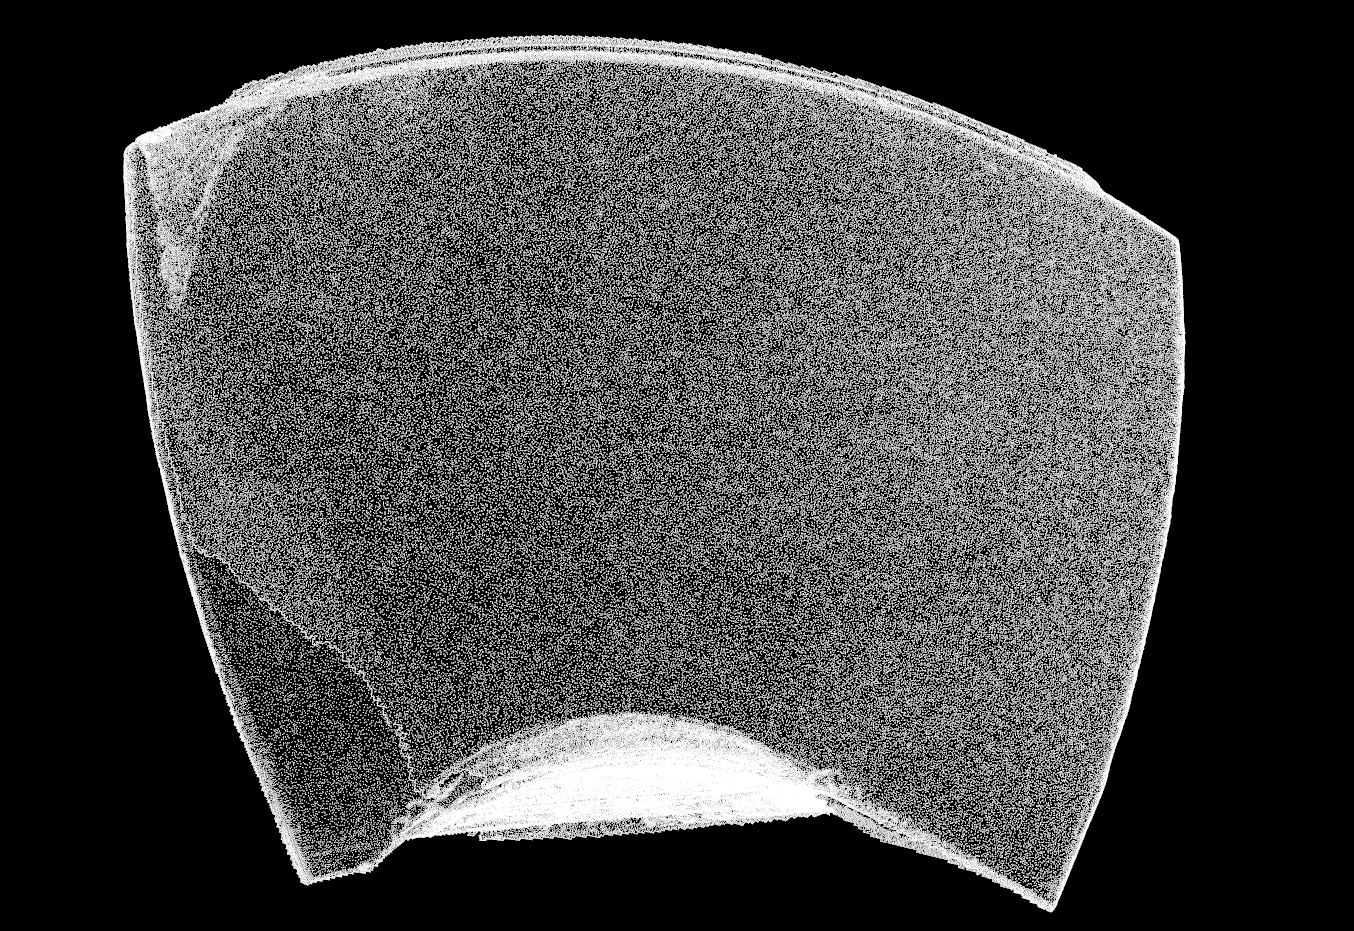
\includegraphics[width=0.9\columnwidth]{figs/calibracao/modelo_pa_faro}
	\caption{Nuvem de pontos da pá aquisitada pelo sensor Faro Focus X330.}
    \label{fig::modelo_pa_faro}
\end{figure}

A identificação da objeto na cena e a estimação da sua posição foi testada em
uma cena de um escritório, como pode ser visualizado na figura
\ref{fig::pa_cena_gen}. O modelo foi sobreposto em vermelho e não houve uma
discrepância visível entre a instância presente na cena e o modelo sobreposto. 
Mesmo com uma diferença de densidade de pontos presente em cada parte da nuvem
de pontos resultante (modelo é muito mais denso que a cena), foi possível
realizar a correta localização do modelo. O ajuste dos paramêtros de
subamostragem necessitaram de maior atenção nesse cenário. Vale ressaltar que o
algoritmo identificou corretamente uma cópia exata do modelo que foi introduzido
na cena, não há presença de ruídos ou oclusões no instância da pá presente na
cena.

\begin{figure}[h!]
	\centering
	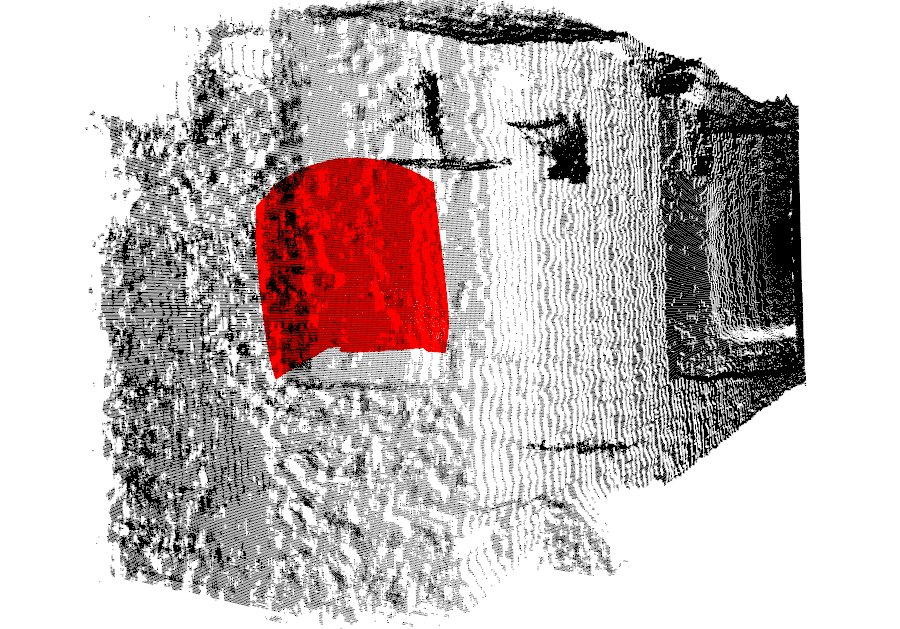
\includegraphics[width=0.9\columnwidth]{figs/calibracao/blade_office5}
	\caption{Exemplo de localização do modelo da pá em uma cena genérica.}
    \label{fig::pa_cena_gen}
\end{figure}

\subsection{Blensor}

A utilização de dados genéricos é útil para a implementação e testes do
algoritmo, entretanto não representa as condições reais que serão encontradas
durante o processo de metalização. A geometria da turbina, da pá, do manipulador
e também as oclusões geradas pelos elementos presentes necessitam ser simulados
para um perfeito ajuste do sistema. Para a simulação desses cenários, foi
utilizado a \textit{toolbox Blensor}\footnotemark
\footnotetext{http://www.blensor.org} baseada no \textit{software} de criação 3D
\textit{Blender}\footnotemark \footnotetext{http://www.blender.org}, o qual
permite a simulação da nuvem de pontos resultante de um sensor em um ambiente
tridimensional. Os objetos inseridos na cena são sólidos 3D, que podem ser
desenhados utilizando-se as ferramentas do próprio programa ou importados de
outros  em outros formatos suportados, como a partir do
Solidworks\textregistered por exemplo. A Figura \ref{fig::blensor_screen}
ilustra a utilização do software, assim como o modelo 3D da turbina importado. A
simulação leva em consideração a distância percorrida pelo pulso emitido, a
intensidade luminosa retornada ao sensor e o tempo decorrido durante o
sensoriamento \cite{Gschwandtner2011}, o que fornece uma melhor aproximação da
resposta do sensor para um ambiente simulado do que simplesmente a utilização de
uma técnica de \textit{raycast} pura.

\begin{figure}[h!]
	\centering
	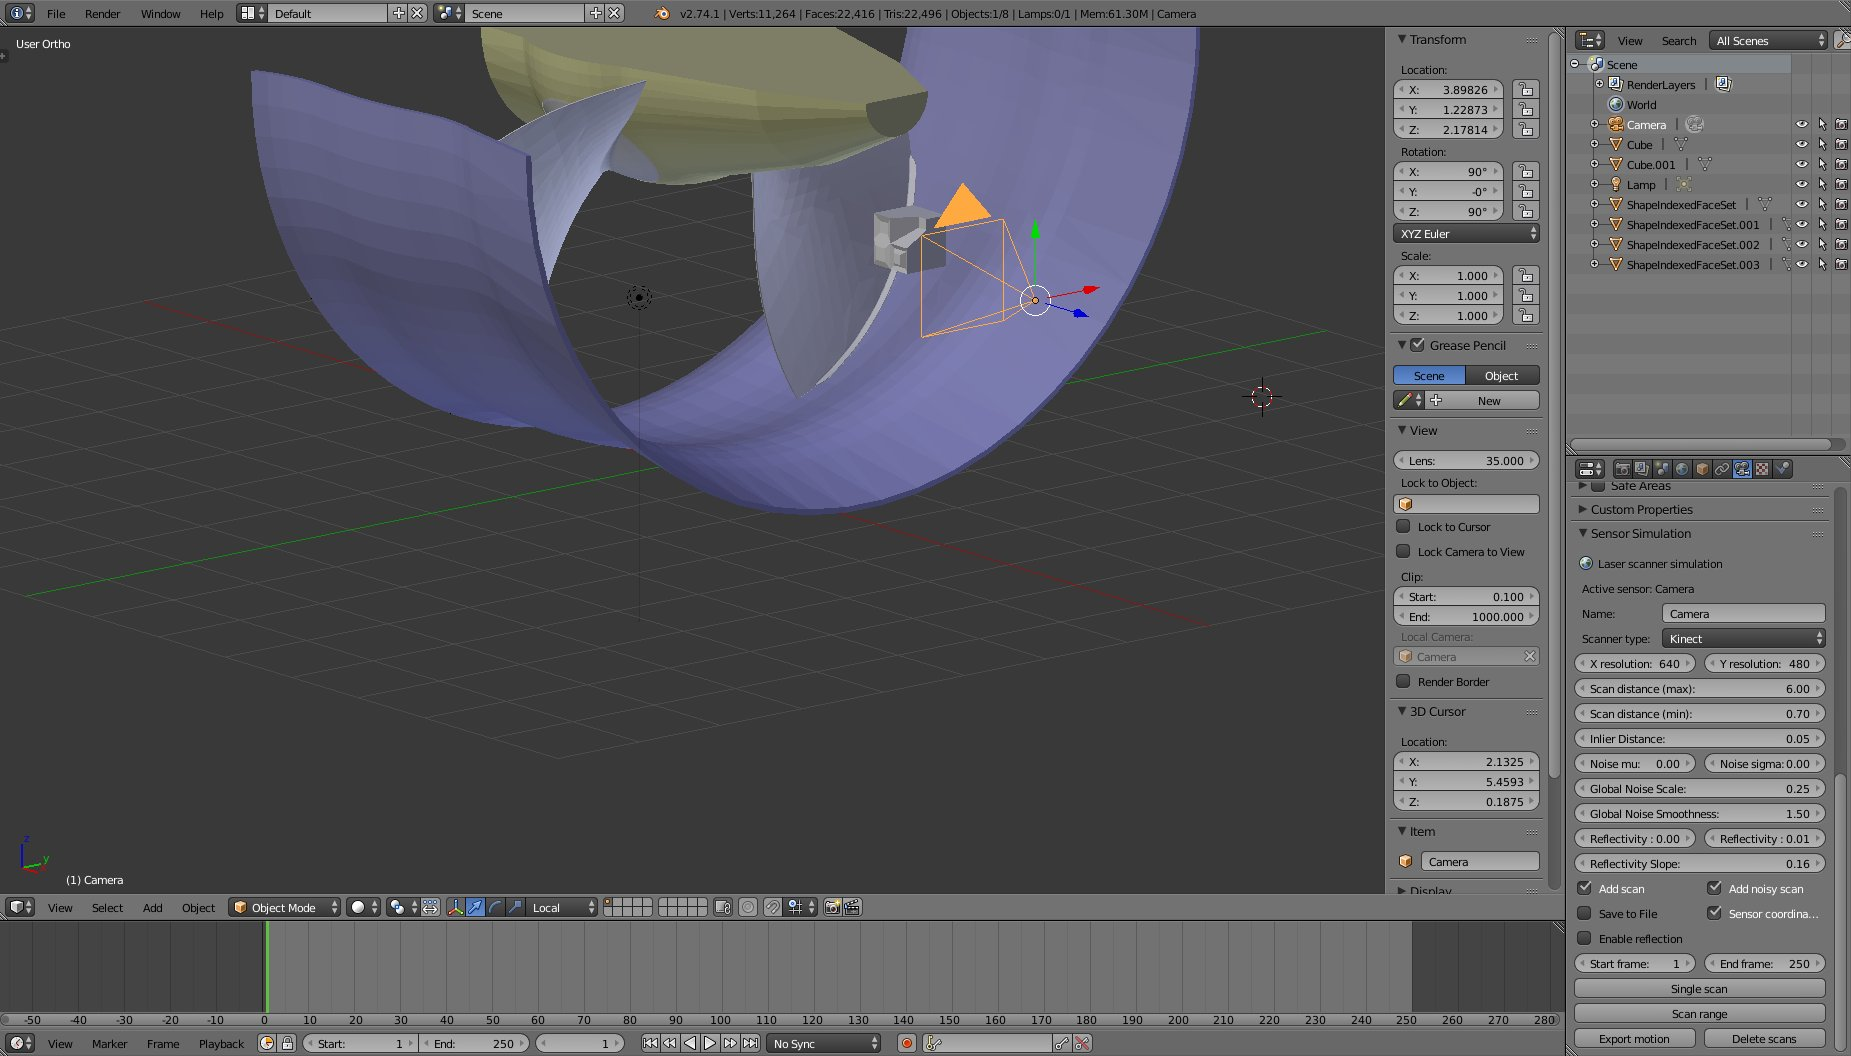
\includegraphics[width=0.9\columnwidth]{figs/calibracao/blensor_screen}
	\caption{Visualização do \textit{Blensor} com o modelo 3D da turbina
	importado.}
    \label{fig::blensor_screen}
\end{figure}

Dentro do ambiente de simulação, é possível a sintetização de dados provenientes
de diversos tipos de sensores laser, como um laserscanner 2D, o sensor
Velodyne e sensores do tipo Kinect. Os parâmetros de configuração
dos sensores também estão disponíveis para ajuste, assim como o nível de ruído. Sensores que não estão
nativamente disponíveis podem ser introduzidos. O sensor Faro Focus X330 não
pertence a lista de sensores previamente carregados pela ferramenta e teve que
ser implementado. As especificações técnicas utilizadas estão de acordo com as
fornecidas pelo fabricante, com exceção do ângulo de visão que foi reduzido para
diminuir o esforço computacional, sem perda de informação. A figura
\ref{fig::blensor_faro} ilustra a resposta simulada do sensor implementado
dentro do ambiente de simulação com a presença do modelo CAD da turbina.


 \begin{figure}[H]
	\centering
	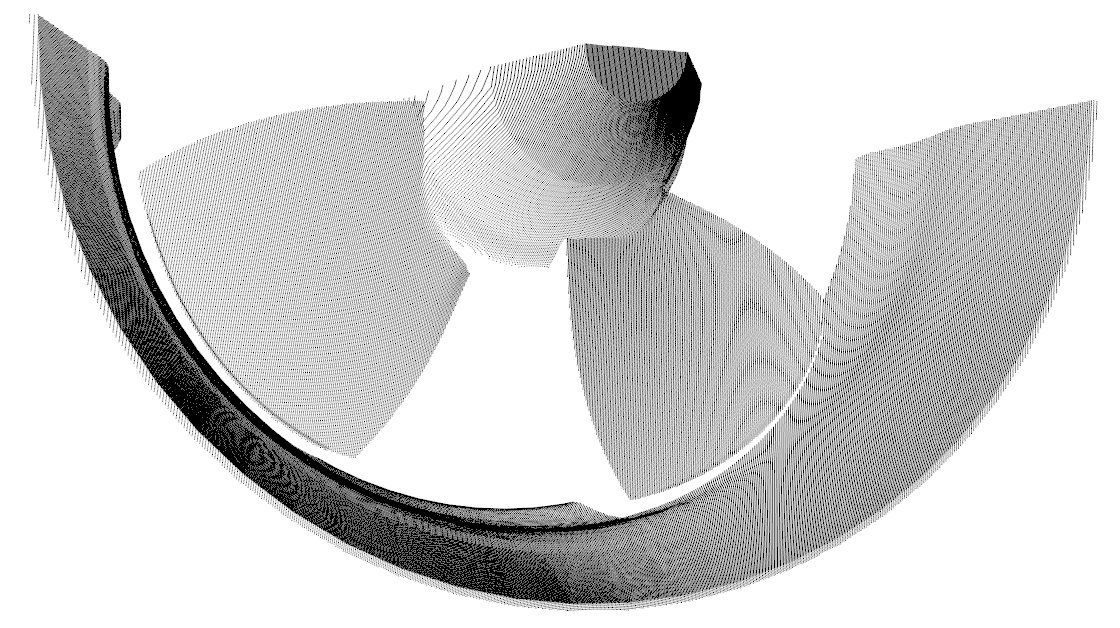
\includegraphics[width=0.9\columnwidth]{figs/calibracao/blensor_faro}
	\caption{Resposta simulada do sensor Faro Focus X330.}
    \label{fig::blensor_faro}
\end{figure}	


Caso seja disponibilizado uma descrição do perfil hidráulico da pá, é possível
também a geração de modelos sem a necessidade de uma inspeção prévia em uma
unidade geradora, na qual haja a presença de dados nas pás, para a aquisição de
dados sobre a turbina. A figura \ref{fig::modelo_pa} ilustra o ambiente de simulação e a
nuvem de pontos final para a criação de um modelo a partir de um arquivo
descritivo. 


\begin{figure}[h!]
	\centering
	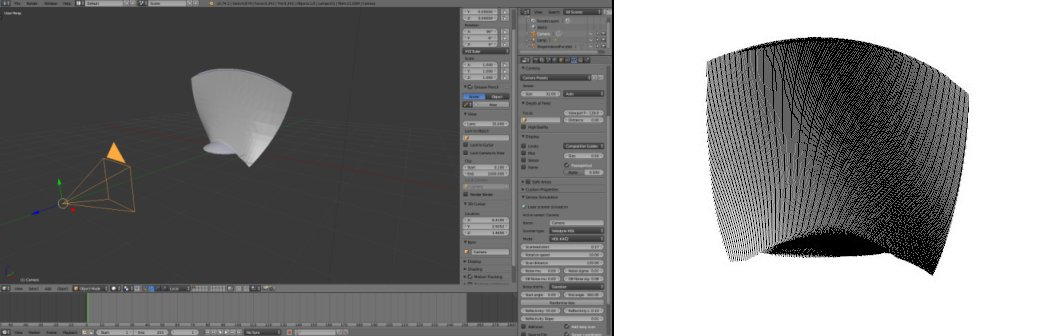
\includegraphics[width=0.9\columnwidth]{figs/calibracao/blensor_pa_sim}
	\caption{Criação de um sensor a partir de um arquivo descritivo da pá.}
    \label{fig::modelo_pa}
\end{figure}

Para representar corretamente as oclusões geradas pelo própria estrutura do
rotor e das pás, é necessário que as cenas sintetizadas a partir da ferramenta
tenham o sensor virtual posicionado em posições que representem os locais no
qual é possível a fixação real do equipamento dentro da UG. As oclusões geradas
pelo sistema de metalização também devem ser previstas e simuladas para um
perfeito ajuste do algoritmo, uma vez que o conjunto do robô e trilhos deve
estar previamente posicionado para que a calibração entre a pá e o efetuador do
manipulador seja realizada. Para isso, o modelo do manipulador MH12 foi
importado para dentro do ambiente de simulação, como ilustrado na figura
\ref{fig::model_mh12} e, em seguida, posicionado entre o sensor e a pá, para
servir de obstáculos para parte dos feixe laser que atingiriam a pá.


\begin{figure}[H]
	\centering
	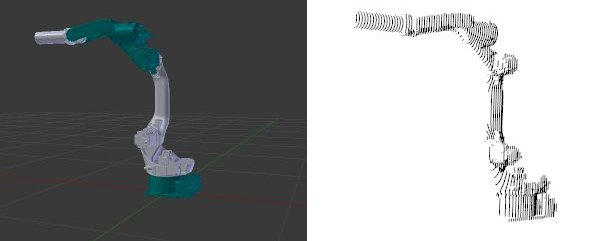
\includegraphics[width=0.9\columnwidth]{figs/calibracao/mh12_model}
	\caption{Visualização do \textit{Blensor} com o modelo 3D da turbina
	importado.}
    \label{fig::model_mh12}
\end{figure}

A Figura \ref{fig::sim_mh12}
ilustra a pá sendo corretamente identificada com a presença do manipulador entre
o sensor e a pá criando uma região de sombra. É possível observar o modelo que
está sendo comparado à cena na parte direita da figura e as linhas verdes
representam as correspondências encontradas entre os descritores do modelo da pá
e os encontrados na cena.

\begin{figure}[H]
	\centering
	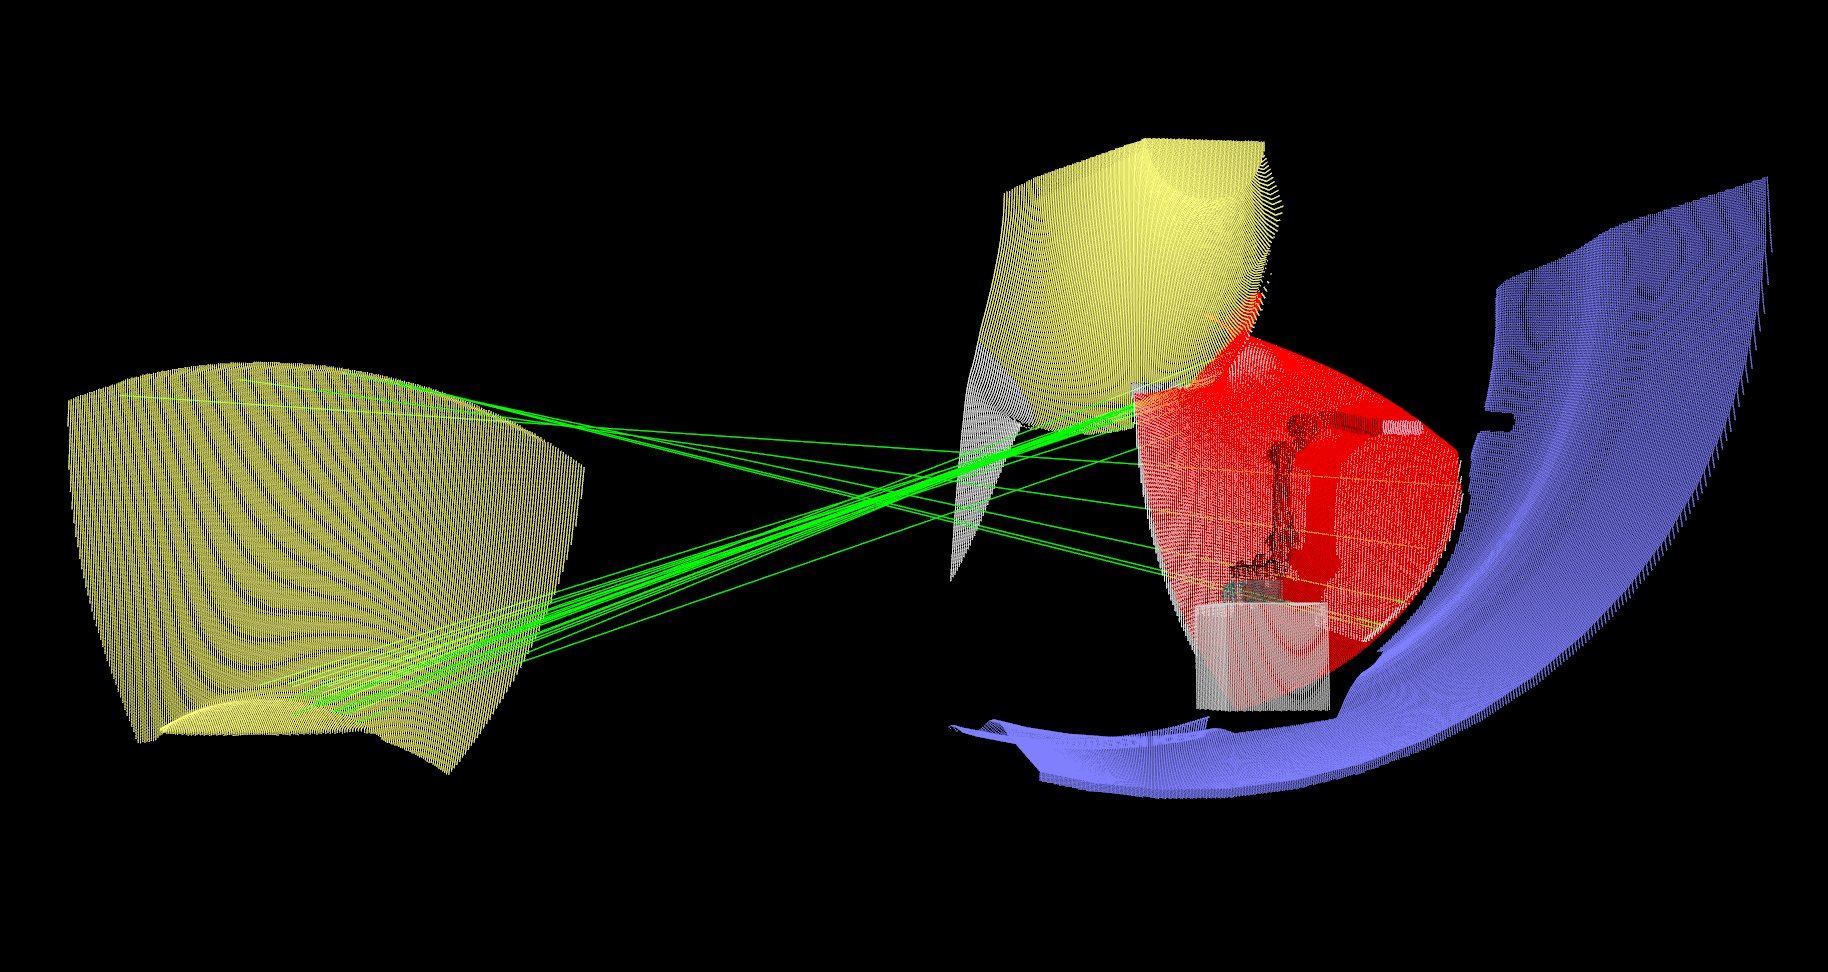
\includegraphics[width=0.9\columnwidth]{figs/calibracao/sim_mh12_sp}
	\caption{Resposta simulada do sensor Faro Focus X330.}
    \label{fig::sim_mh12}
\end{figure}	

\section{Conclusão}
%TODO TODOS: conclusoes finais

% -.-.-.-.-.-.-.-.-.-.-.-.-.-.-.-.-.-.-.-.-.-.-.-.-.-.-.-.-.-.-.-.-.-.-.-.-.-.-.
%Mecânica
As simulações pelo Método de Elementos Finitos verificaram a rigidez da
estrutura dada, a geometria imposta pelo conceito P-R-P-P e para as opções
comerciais disponíveis de material, perfil de alumínio estrutural, trilho e bases
magnéticas.
Os resultados se mostraram satisfatórios para os os componentes selecionados,
ressaltando que foram considerados casos extremos de operação. A flexibilidade
da estrutura causa erros com ordem de grandeza de $1~mm$, o que não interfere na
qualidade do processo.
As forças resultantes nos pontos de ancoragem permitem dimensionamento e seleção
das bases mecânicas para cada região de ancoragem, não limitando o mesmo tamanho
de base para todos os pontos.
Os resultados de integridade do componentes conferiram Fatores de Segurança
aceitáveis e dentro dos valores recomendados para projetos mecânicos em geral.
% -.-.-.-.-.-.-.-.-.-.-.-.-.-.-.-.-.-.-.-.-.-.-.-.-.-.-.-.-.-.-.-.-.-.-.-.-.-.-.

  
\bibliography{main,calibracao}
\appendix
\section{Apêndice A: Relatório de simulação do trilho}\label{ape::magnetic}

Neste apêndice apresenta-se a íntegra do relatório de resultado gerado pelo
programa \textit{SKF Linear Guide Calculator} de análise de carregamentos e 
Fator de Segurança para os trilhos SKF.

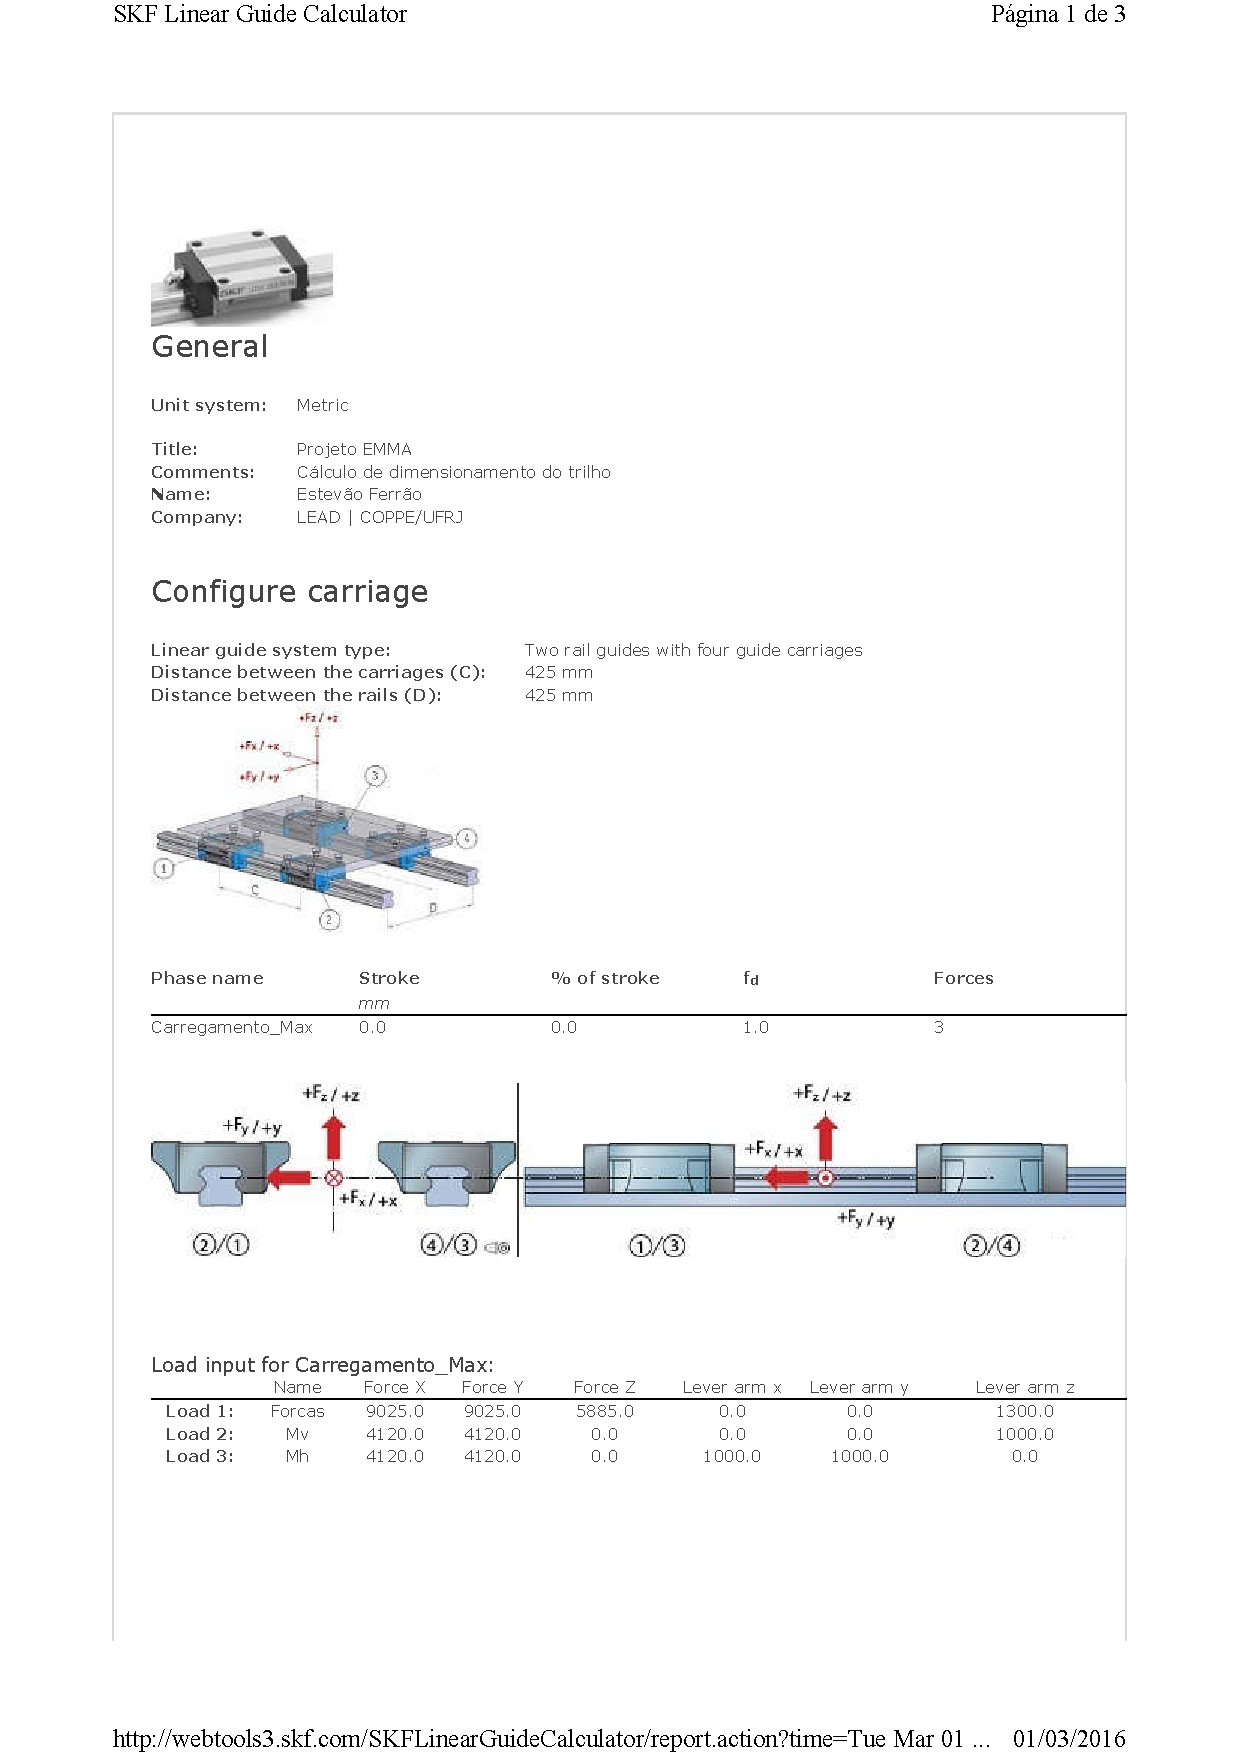
\includepdf[pages=1-,scale=0.9]{apendice/Report_SKF.pdf}
\end{document}
